\documentclass{article}
\usepackage{pdfpages}

\title{Research Portfolio}
\author{Hector Bahamonde}
\date{\today}

\usepackage{hyperref}
\hypersetup{
    colorlinks,
    citecolor=blue,
    filecolor=blue,
    linkcolor=blue,
    urlcolor=blue
}


\pagenumbering{gobble} % no page number




\begin{document}

\maketitle
 
\tableofcontents


\vspace{1cm}
\dotfill

\newpage

% Research Statement
%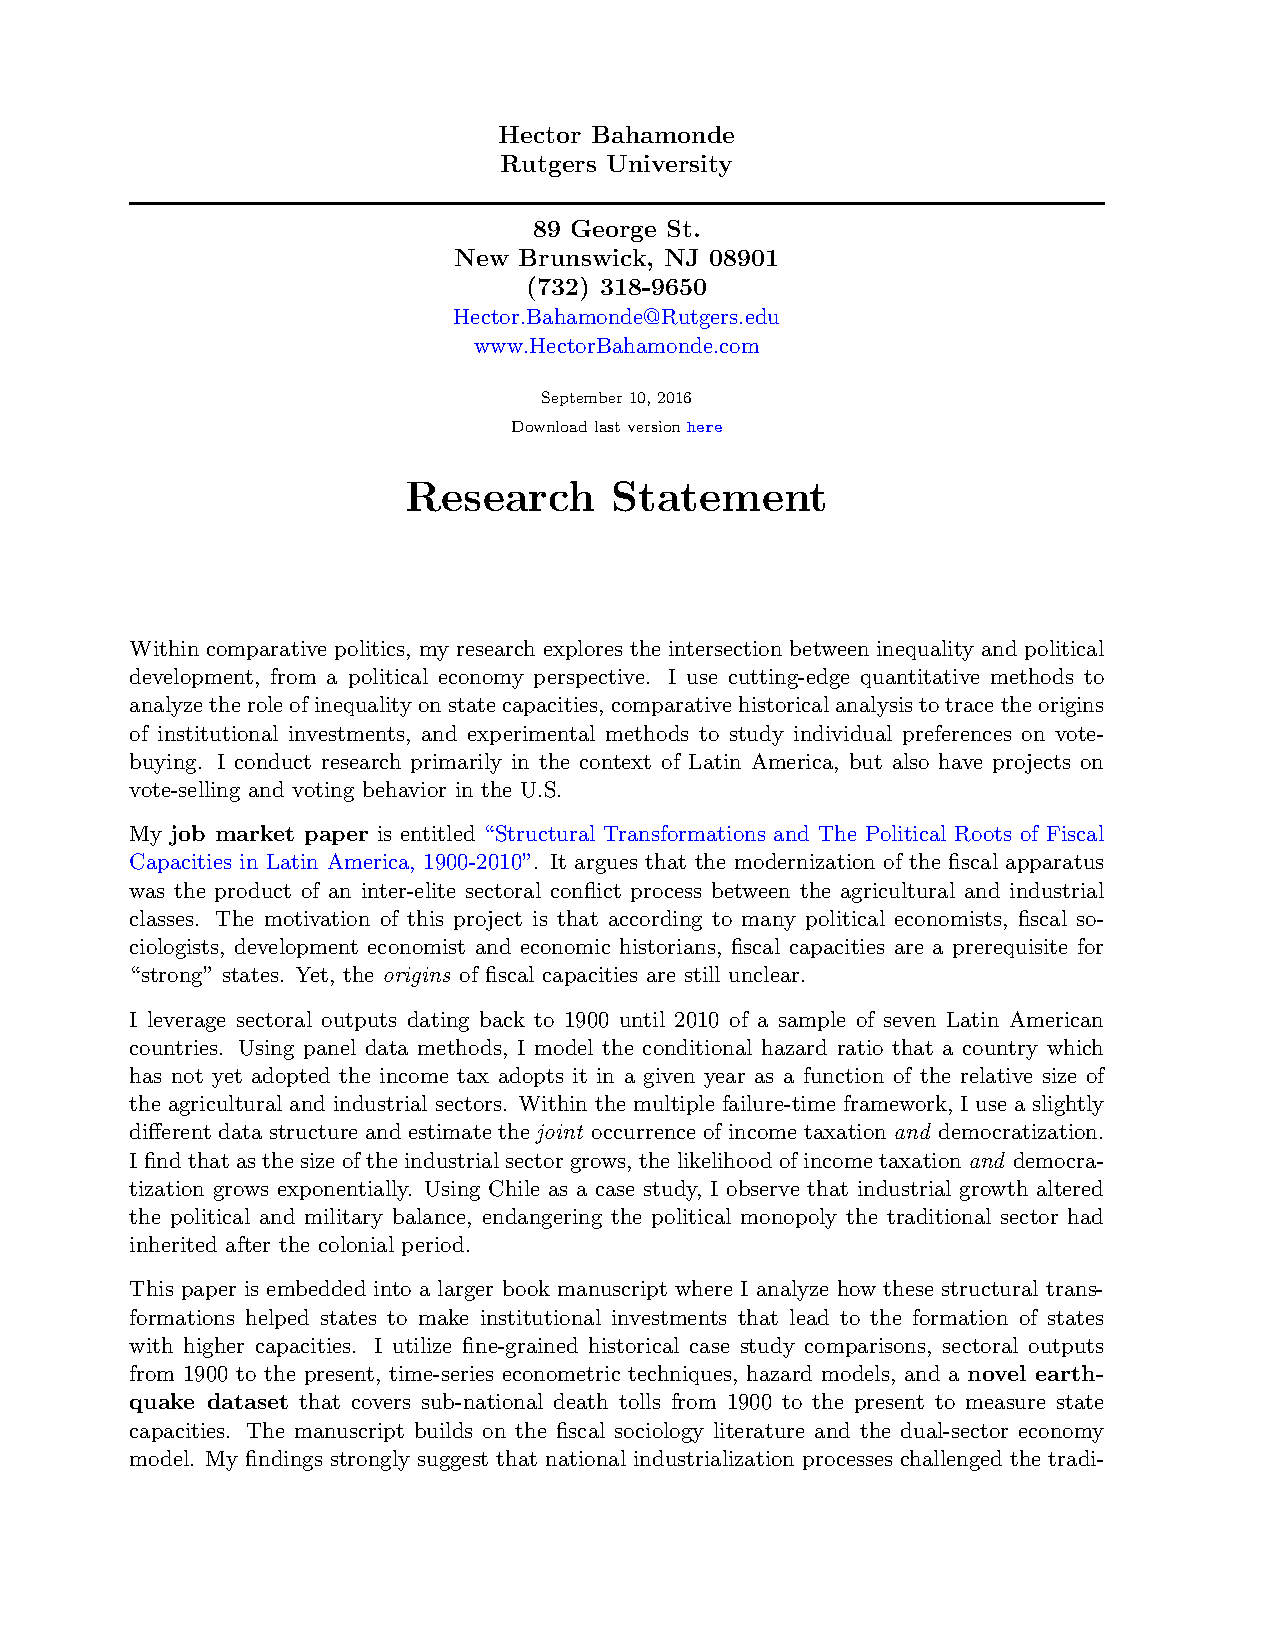
\includepdf[pages=-,addtotoc={1,section,1,Research Statement,Research Statement}, pagecommand={\phantomsection{}{}}]{/Users/hectorbahamonde/RU/Job_Market/Bahamonde_Research_Statement.pdf}


% Job Market Paper
\includepdf[pages=-,addtotoc={1,section,1,Job Market Paper: Income Taxation and State Capacities,Job Market Paper: Income Taxation and State Capacities}, pagecommand={\phantomsection{}{}}]{/Users/hectorbahamonde/RU/Dissertation/Papers/Earthquake_Paper/Bahamonde_Earthquake_Paper.pdf}

% Sectoral Origins of Income Taxation
\includepdf[pages=-,addtotoc={1,section,1,Additional Paper 1: Sectoral Origins of Income Taxation,Sectoral Origins of Income Taxation}, pagecommand={\phantomsection{}{}}]{/Users/hectorbahamonde/RU/Dissertation/Papers/IncomeTaxAdoption/Bahamonde_IncomeTaxAdoption.pdf}


% Clientelistic Targeting in Brazil
\includepdf[pages=-,addtotoc={1,section,1,Additional Paper 2: Clientelistic Targeting in Brazil,Clientelistic Targeting in Brazil}, pagecommand={\phantomsection{}{}}]{/Users/hectorbahamonde/RU/research/Clientelism_paper/Bahamonde_Clientelism_Paper.pdf}


% Sectoral Competition and Political Development
\includepdf[pages=-,addtotoc={1,section,1,Additional Paper 3: Sectoral Competition and Political Development,Sectoral Competition and Political Development}, pagecommand={\phantomsection{}{}}]{/Users/hectorbahamonde/RU/Dissertation/Papers/NegativeLink/Bahamonde_NegativeLink.pdf}


\end{document}







